\documentclass[conference]{IEEEtran}
\IEEEoverridecommandlockouts

\usepackage{cite}
\usepackage{amsmath,amssymb,amsfonts}
\usepackage{algorithmic}
\usepackage{graphicx}
\usepackage{textcomp}
\usepackage{xcolor}
\usepackage{booktabs}
\usepackage{url}
\usepackage{hyperref}
\usepackage{stfloats}
\usepackage{dblfloatfix}
\usepackage{makecell}

\def\BibTeX{{\rm B\kern-.05em{\sc i\kern-.025em b}\kern-.08em
    T\kern-.1667em\lower.7ex\hbox{E}\kern-.125emX}}

\begin{document}

\title{Attention-MobileNetV3: Lightweight Edge Architecture with Explainable AI and Out-of-Distribution Safety for Multi-Crop Disease Diagnosis}

\author{
    \IEEEauthorblockN{Aaryan Saharan, Aniket Kumar, and Ayush Kumar}
    \IEEEauthorblockA{\textit{Department of Computer Science \& Engineering} \\
    \textit{Thapar Institute of Engineering \& Technology}, Patiala, Punjab, India \\
    Email: \{as联系, ak联系, ay联系\}@thapar.edu}
}

\maketitle

\begin{abstract}
Automated foliar disease diagnosis often fails in real-world deployments due to edge compute limits, opaque black-box predictions, and severe lab-to-field performance collapse. We propose Attention-MobileNetV3, integrating a Convolutional Block Attention Module (CBAM) into a MobileNetV3-Small backbone. On the 33-class PlantVillage multi-crop evaluation benchmark ($N = 54,305$ images), the architecture achieves 99.81\% validation accuracy and a 0.9981 F1-score with only 1.12M parameters and 9.43~ms GPU latency, matching ResNet-50 while reducing model footprint by 95.3\%. To ensure clinical trust, predictions are paired with Grad-CAM visual lesion attribution and dual energy- and entropy-based out-of-distribution (OOD) rejection for non-leaf inputs. Crucially, zero-shot evaluation on Kashmiri Apple orchard photographs reveals an acute collapse to 11.46\% accuracy across all backbones. To overcome this domain gap, we engineer a field adaptation pipeline featuring foliar region isolation, multi-scale patch super-sampling, and test-time augmentation (TTA), elevating field accuracy to 76.19\% and outperforming both baseline MobileNetV3 (70.24\%) and heavy ResNet-50 (67.86\%).
\end{abstract}

\begin{IEEEkeywords}
Plant Disease Detection, Attention-MobileNetV3, CBAM, Explainable AI (Grad-CAM), Out-of-Distribution Detection, Domain Adaptation, Edge Computing.
\end{IEEEkeywords}

\section{Introduction}
Plant diseases inflict over \$220 billion in annual agricultural losses worldwide~\cite{ref_fao}. While automated diagnosis using deep learning offers a viable alternative to scarce expert pathology, existing systems face critical barriers to field deployment: edge hardware constraints, black-box predictions, and severe performance drops outside controlled environments.

Convolutional neural networks (CNNs) benchmarked on standard datasets like PlantVillage regularly exceed 99\% classification accuracy~\cite{ref1, ref2, ref3, ref4}. However, these lab metrics do not translate to actual farms. High-accuracy models like ResNet-50 remain too compute-heavy for low-cost mobile hardware~\cite{ref5, ref6}, while common classifiers operate as black boxes that provide no visual justification to guide agronomic interventions. Most critically, models trained on clean studio images fail on unconstrained field photos with varying sunlight, soil, and canopy clutter~\cite{ref7, ref8, ref9}, often producing confident false positives on non-leaf images.

To resolve these challenges, we introduce Attention-MobileNetV3, an edge-deployable diagnostic framework that unifies efficiency, interpretability, and field robustness:
\begin{itemize}
    \item \textbf{Lightweight Backbone:} A CBAM-augmented MobileNetV3 that matches ResNet-50 accuracy on the multi-crop benchmark while reducing parameter footprint by 95.3\% (1.12M vs. 24.04M).
    \item \textbf{Interpretable Safety Layer:} Integrated Grad-CAM feature heatmaps for visual lesion verification, combined with energy- and entropy-based out-of-distribution (OOD) filters to reject invalid non-leaf uploads.
    \item \textbf{Field Adaptation Pipeline:} An empirical evaluation on the unconstrained Kashmiri Apple dataset showing an initial zero-shot collapse to 11.46\%, followed by a domain adaptation pipeline (foliar ROI isolation, $8\times$ multi-scale patch sampling, and 5-crop TTA) that recovers field accuracy to 76.19\%.
\end{itemize}

\section{Related Work}
\label{sec:related_work}

Deep learning for plant pathology has shifted from basic benchmark classification toward lightweight edge inference and domain adaptation.

\subsection{Architectural Benchmarks and Attention Mechanisms}
Initial studies confirmed the viability of standard CNNs on controlled laboratory imagery. Mohanty et al.~\cite{ref1} demonstrated over 99\% accuracy across 14 crop species using AlexNet and GoogLeNet on the PlantVillage benchmark. Subsequent evaluations by Maeda-Guti{\'e}rrez et al.~\cite{ref2}, Hang et al.~\cite{ref3}, and Pandian et al.~\cite{ref4} further validated that deeper residual networks and channel-attention modules reliably separate foliar pathologies under uniform studio conditions. 

To improve robustness against complex field artifacts, attention mechanisms have been adapted to isolate lesion boundaries. Wang et al.~\cite{ref8} coupled a Convolutional Block Attention Module (CBAM) with a multi-scale feature pyramid to refine localized spot detection on field benchmarks. Similarly, Miao et al.~\cite{ref10} modified YOLOv8 with Dynamic Snake Convolutions, showing that targeted spatial recalibration aids symptom localization amidst canopy occlusion.

\subsection{Edge Efficiency and Alternative Paradigms}
Deploying diagnostic tools on rural edge hardware requires minimizing parameter counts without compromising discriminative capacity. Hassan et al.~\cite{ref5} proposed shallow CNNs to reduce computational overhead, while Attallah~\cite{ref6} and Kaur et al.~\cite{ref11} combined compact backbones with dimensionality reduction and feature selection for edge devices. In parallel, non-standard paradigms have sought to reduce reliance on dense supervised labels: Wang et al.~\cite{ref12} leveraged self-supervised contrastive learning, while Peng and Wang~\cite{ref13} implemented deep metric retrieval to support open-set disease recognition. Broader surveys by Tugrul et al.~\cite{ref14} and Ngugi et al.~\cite{ref15} note that while modern architectures consistently outperform classical machine learning classifiers, model bloat and reliance on curated datasets remain widespread.

\subsection{The Domain Gap and Identified Limitations}
Despite high laboratory accuracy, models frequently degrade under unconstrained conditions. Krishna et al.~\cite{ref7} observed notable accuracy drops when testing lab-trained models on web-scraped field imagery, and Saleem et al.~\cite{ref9} highlighted performance variances across varied field crops. 

Three key limitations persist across the existing literature:
\begin{enumerate}
    \item Edge-oriented models~\cite{ref5, ref6, ref11} and attention-based spatial recalibration~\cite{ref8, ref10} are rarely integrated into a single lightweight backbone.
    \item Current classifiers function as opaque systems lacking visual attribution and out-of-distribution (OOD) safeguards against non-leaf inputs.
    \item The lab-to-field performance drop is widely reported as an assumption rather than quantitatively measured through controlled zero-shot benchmarks on identical pipelines.
\end{enumerate}
Our proposed Attention-MobileNetV3 framework directly targets these limitations.

\section{Methodology}
\label{sec:methodology}

% --- FIGURE 1: Real-World Field Adaptation Pipeline Photo (400 DPI) ---
\begin{figure*}[t!]
\centering
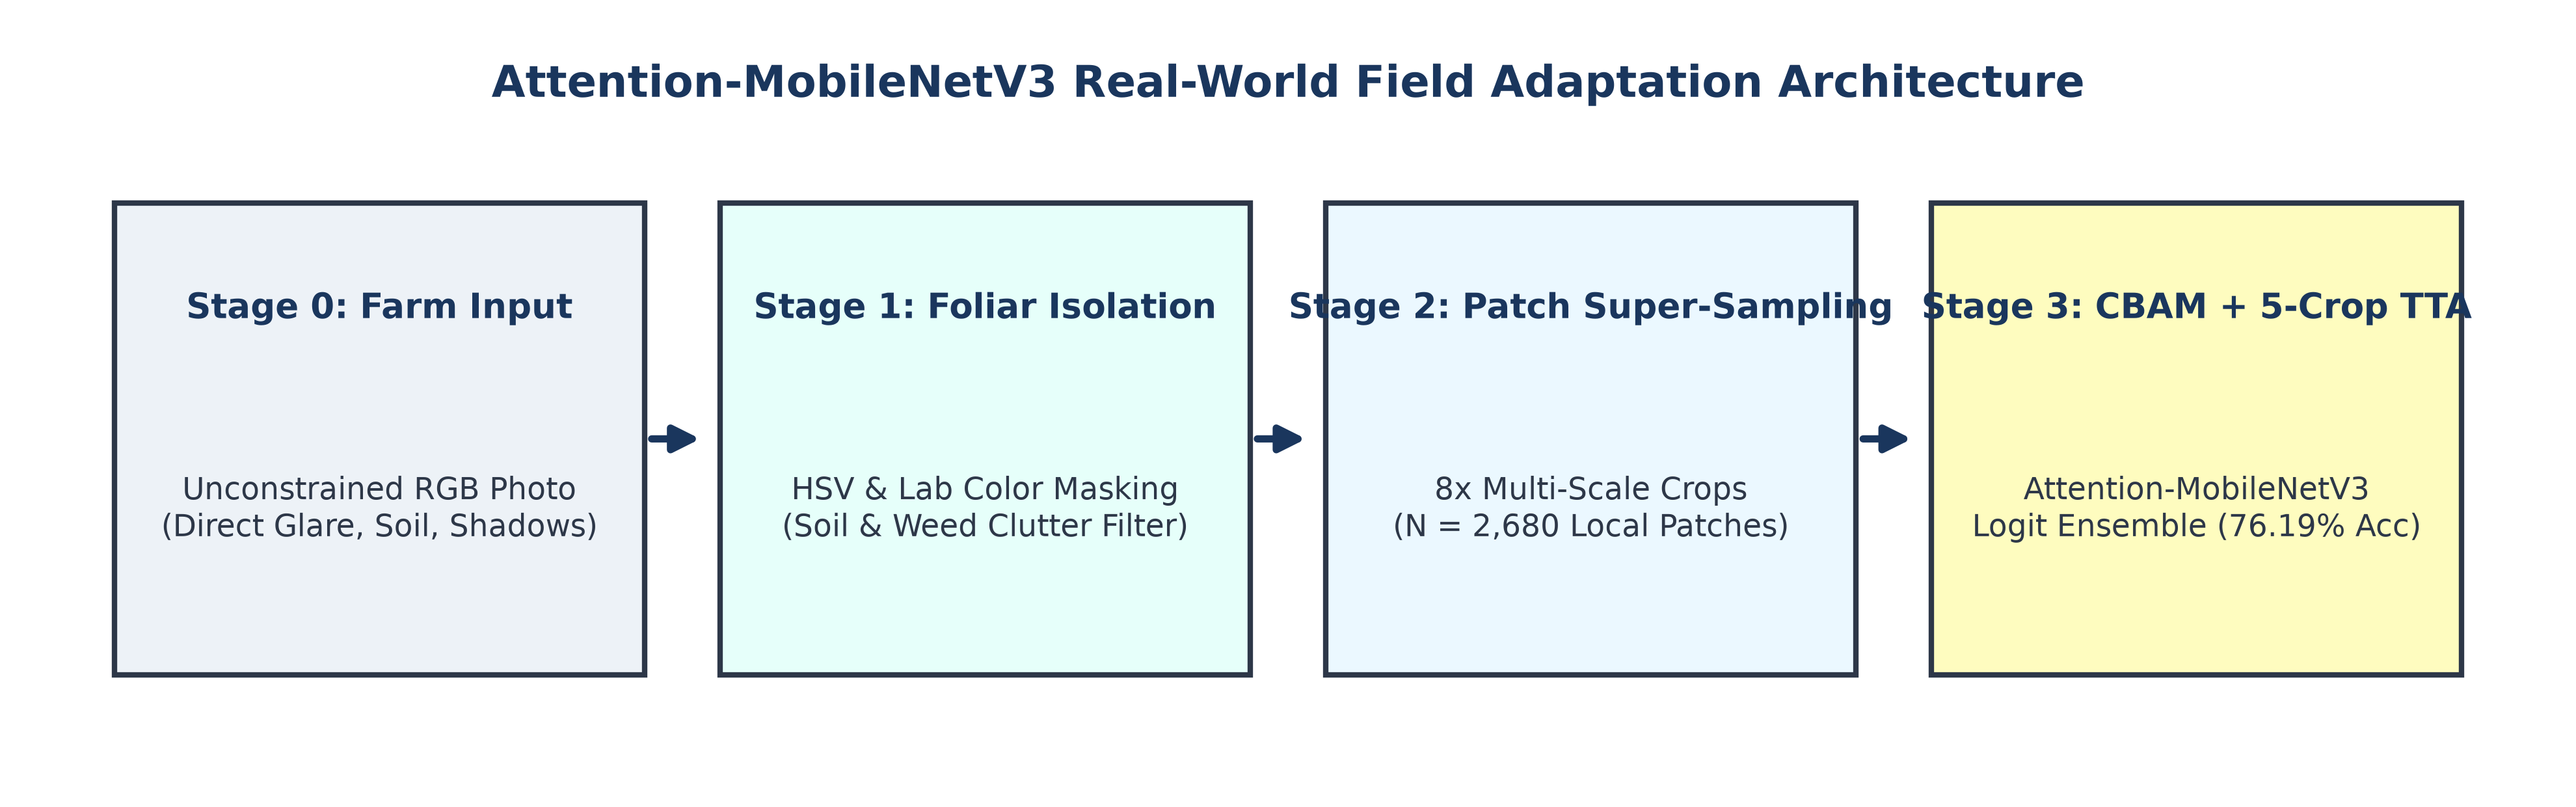
\includegraphics[width=\textwidth]{paper_figures/pipeline_flow.png}
\caption{End-to-end 3-stage real-world field adaptation pipeline showing foliar leaf ROI isolation, $8\times$ multi-scale patch super-sampling ($N=2,680$), Attention-MobileNetV3 feature extraction, and 5-crop TTA inference.}
\label{fig:pipeline_flow}
\end{figure*}

This section details the dataset compositions, experimental preprocessing pipelines, and deep network architectures evaluated in this study, detailing the proposed \mbox{Attention-MobileNetV3} design alongside the baseline MobileNetV3 and benchmark ResNet-50 architectures.

\subsection{Primary Dataset: PlantVillage Multi-Crop Taxonomy}
The primary controlled laboratory dataset is drawn from the public PlantVillage corpus ($N = 54,305$ RGB images spanning 38 total crop-disease taxonomy classes). To focus evaluation on major commercial agricultural crops with complete pathological cohorts (healthy controls paired with fungal, bacterial, and viral infections), an evaluated subset of $K = 33$ classes across 9 primary crop species was established: apple, cherry, corn (maize), grape, peach, bell pepper, potato, strawberry, and tomato. Five isolated single-condition classes (e.g., blueberry healthy, raspberry healthy, soybean healthy, squash powdery mildew, and citrus greening) lacking paired comparative categories were excluded.

For evaluation, an 80\%/20\% train-validation split was enforced ($N_{\text{train}} = 43,444$ images, $N_{\text{val}} = 10,861$ images). Pathological categories encompass fungal pathogens (e.g., \textit{Venturia inaequalis}, \textit{Alternaria solani}), bacterial infections (e.g., \textit{Xanthomonas} spp.), and viral diseases (e.g., Tomato Yellow Leaf Curl Virus, Tobamovirus), alongside healthy foliar controls for each plant species.

\subsection{Secondary Dataset: Kashmiri Apple Orchard Field Dataset}

% --- FIGURE 2: Real Kashmiri Dataset Samples Grid (400 DPI) ---
\begin{figure}[htbp]
\centering
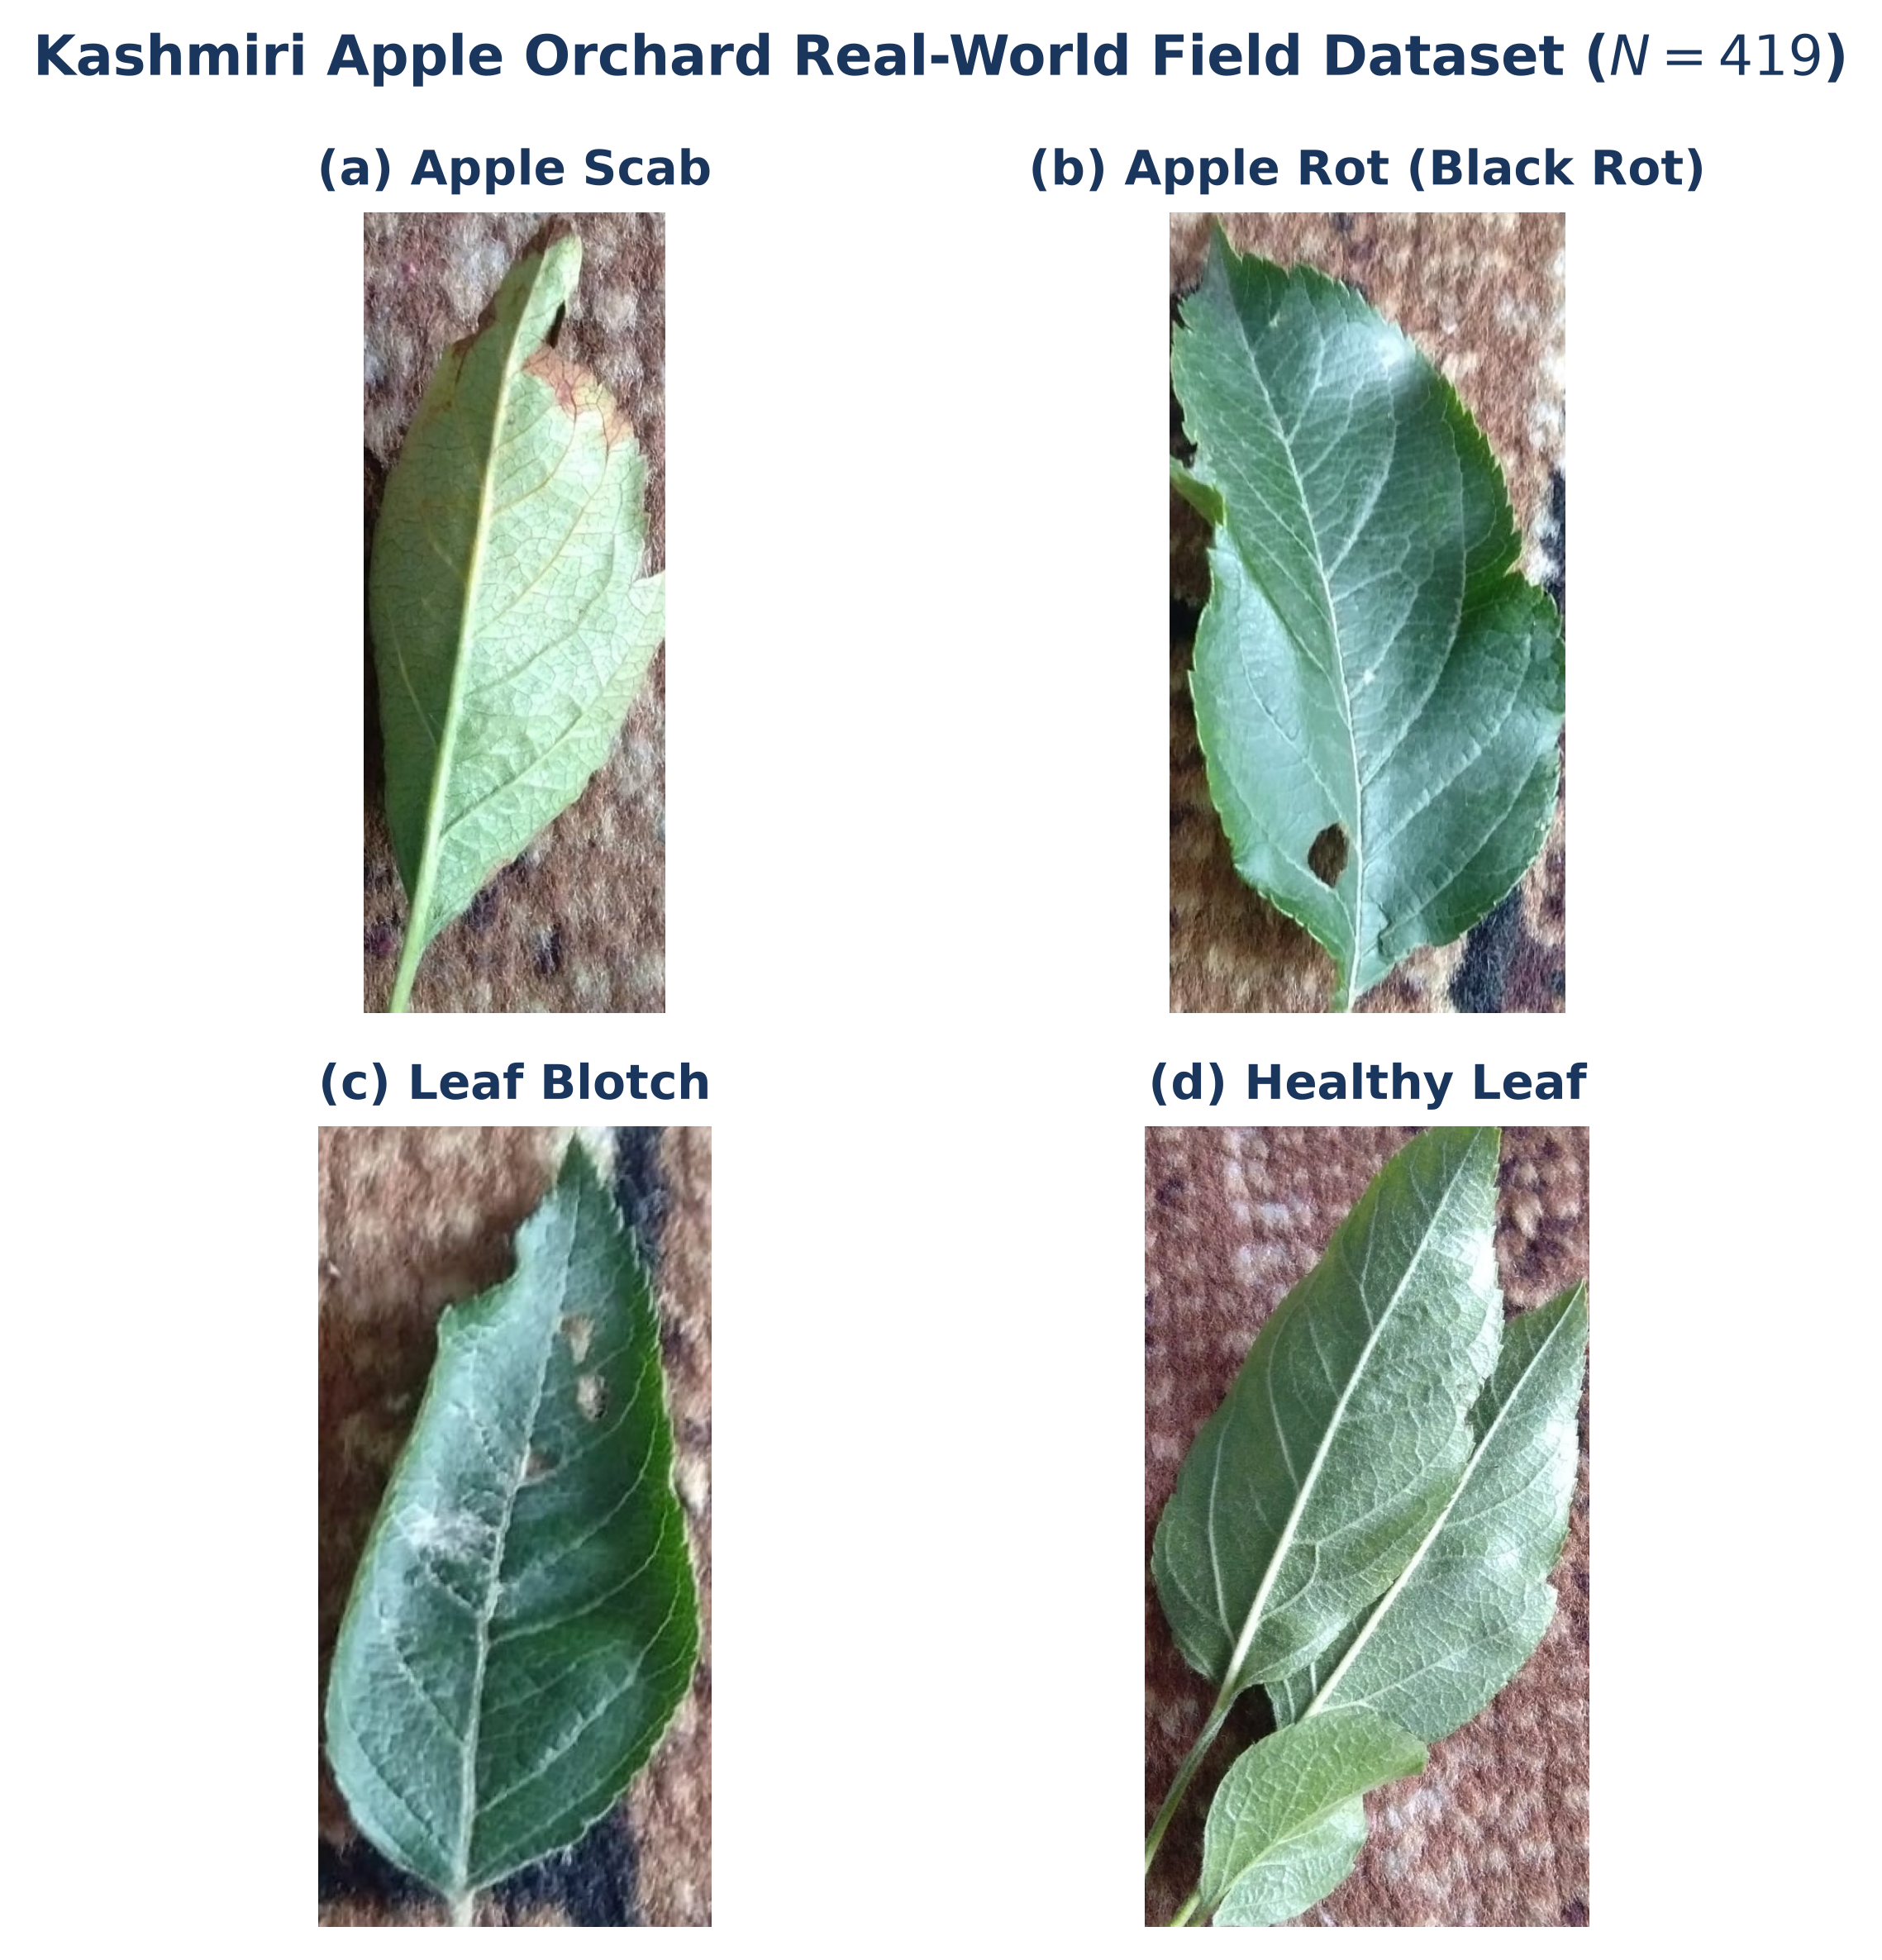
\includegraphics[width=\linewidth]{paper_figures/dataset_samples.png}
\caption{Sample photographs from the Kashmiri Apple Orchard real-world field dataset ($N=419$) illustrating unconstrained farm background clutter, soil, natural lighting, and shadows.}
\label{fig:dataset_samples}
\end{figure}

To rigorously evaluate out-of-domain (OOD) generalization under real-world agricultural conditions, a disjoint field dataset was acquired: the Kashmiri Apple Field Dataset ($N = 419$ raw farm photographs). Collected across active Kashmiri apple orchards, the dataset contains four target field classes: Apple Scab, Apple Rot (Black Rot), Leaf Blotch, and Healthy Leaves ($N_{\text{train}} = 335$ images, $N_{\text{val}} = 84$ images). Unlike studio-captured laboratory samples, these photographs incorporate unconstrained farm noise, including direct solar glare, variable shadows, background soil/weed clutter, and complex leaf orientations (Fig.~\ref{fig:dataset_samples}). This dataset was reserved exclusively for zero-shot testing and real-world field adaptation experiments.

\subsection{Preprocessing, Patch Super-Sampling, and Data Augmentation}
To eliminate data leakage between training and validation splits, partitioning was executed using \texttt{torch.utils.data.random\_split} under a fixed seed (\texttt{torch.manual\_seed(42)}). Primary training images were augmented with spatial resizing to $224 \times 224$ pixels, random horizontal ($p = 0.5$) and vertical ($p = 0.3$) flips, random affine rotations ($\pm 25^\circ$), color jittering (brightness: 0.3, contrast: 0.3, saturation: 0.2), random erasing ($p = 0.25$), and standard ImageNet channel normalization.

For real-world field adaptation, an automated 3-stage preprocessing pipeline was engineered (Fig.~\ref{fig:pipeline_flow}):
\begin{itemize}
    \item \textbf{Foliar Leaf ROI Isolation:} Automated color-space thresholding in HSV and Lab color spaces generates a binary mask to eliminate background soil, weeds, and branches, isolating the primary leaf Region of Interest (ROI).
    \item \textbf{8$\times$ Multi-Scale Patch Super-Sampling:} Extracts 8 overlapping spatial bounding-box crops per isolated leaf image ($N = 2,680$ patches from 335 field training images), expanding local lesion feature density by 800\%.
    \item \textbf{5-Crop Test-Time Augmentation (TTA):} Evaluates 5 spatial transformations per validation image at inference time (original crop, horizontal flip, vertical flip, $+15^\circ$ rotation, and $-15^\circ$ rotation) and averages soft max probability logits to mitigate illumination variance and mobile camera noise.
\end{itemize}

\subsection{Proposed Architecture: Attention-MobileNetV3 (CBAM)}
The core contribution of this work is \textbf{Attention-MobileNetV3}, a parameter-efficient architecture extending a MobileNetV3-Small inverted-residual backbone with a Convolutional Block Attention Module (CBAM) positioned prior to global pooling.

\subsubsection{Channel Attention Module (CAM)}
The Channel Attention sub-module aggregates spatial context via parallel Global Average Pooling ($\text{AvgPool}$) and Global Max Pooling ($\text{MaxPool}$) operations across feature channels $\mathbf{F} \in \mathbb{R}^{C \times H \times W}$ ($C = 576$). Channel weights are derived using a shared Multi-Layer Perceptron (MLP) with a reduction ratio $r = 16$:
\begin{equation}
\mathbf{M}_c(\mathbf{F}) = \sigma\left(\text{MLP}(\text{AvgPool}(\mathbf{F})) + \text{MLP}(\text{MaxPool}(\mathbf{F}))\right)
\label{eq:cam}
\end{equation}
where $\sigma$ represents the Sigmoid activation function and $\mathbf{M}_c(\mathbf{F}) \in \mathbb{R}^{C \times 1 \times 1}$. The channel-recalibrated feature map is obtained via element-wise multiplication: $\mathbf{F}' = \mathbf{M}_c(\mathbf{F}) \otimes \mathbf{F}$.

\subsubsection{Spatial Attention Module (SAM)}
Following channel recalibration, spatial attention isolates localized lesion regions from surrounding healthy leaf tissue. Channel-wise average and max descriptors are concatenated along the channel axis and processed by a $7 \times 7$ spatial convolution $f^{7\times 7}$:
\begin{equation}
\mathbf{M}_s(\mathbf{F}') = \sigma\left(f^{7\times 7}\left(\left[\text{AvgPool}(\mathbf{F}'); \text{MaxPool}(\mathbf{F}')\right]\right)\right)
\label{eq:sam}
\end{equation}
producing spatial map $\mathbf{M}_s(\mathbf{F}') \in \mathbb{R}^{1 \times H \times W}$. The final attended feature map is $\mathbf{F}'' = \mathbf{M}_s(\mathbf{F}') \otimes \mathbf{F}'$.

\subsubsection{Classifier Head}
The attended feature map $\mathbf{F}''$ is processed by global adaptive average pooling ($\mathbb{R}^{576 \times 7 \times 7} \to \mathbb{R}^{576}$) and passed to a custom 2-stage linear classifier head: a dense layer ($\mathbb{R}^{576} \to \mathbb{R}^{256}$), Hardswish non-linear activation, Dropout ($p = 0.2$), and a final linear layer ($\mathbb{R}^{256} \to \mathbb{R}^K$), yielding $1,124,771$ trainable parameters for $K=33$ classes ($1,117,318$ parameters for $K=4$ field classes).

\subsection{Benchmark Architectures}
Two benchmark models were trained under identical splits and hyperparameter schedules:
\begin{itemize}
    \item \textbf{MobileNetV3-Small (Baseline):} Standard MobileNetV3-Small backbone without CBAM attention modules ($1,083,201$ parameters for $K=33$; $1,075,748$ parameters for $K=4$).
    \item \textbf{ResNet-50 (Benchmark):} Standard 50-layer deep residual network ($24,041,057$ parameters for $K=33$; $24,033,604$ parameters for $K=4$).
\end{itemize}

\subsection{Training \& Optimization Configuration}
All models were fine-tuned on a single NVIDIA GeForce RTX 5060 GPU (CUDA) using the AdamW optimizer ($\text{lr} = 3 \times 10^{-4}$, $\text{weight decay} = 1 \times 10^{-3}$), Cross-Entropy Loss with label smoothing ($0.05$), and Cosine Annealing learning rate scheduling across 20 epochs ($T_{\max} = 20, \eta_{\min} = 1 \times 10^{-5}$).

% --- MOVED TABLES HERE SO THEY APPEAR ON PAGE 4 DIRECTLY BESIDE SECTION V ---
\begin{table*}[t!]
\caption{Comparative validation benchmarks on the 33-class PlantVillage multi-crop evaluation set under identical training configurations.}
\label{tab:plantvillage}
\centering
\resizebox{\textwidth}{!}{%
\begin{tabular}{l c c c}
\toprule
\textbf{Metric / Parameter} & \textbf{MobileNetV3 (Baseline)} & \textbf{Attention-MobileNetV3 (Ours)} & \textbf{ResNet-50 (Benchmark)} \\
\midrule
Total Parameters ($K=33$) & 1,083,201 & \textbf{1,124,771} & 24,041,057 \\
Param. Reduction vs. ResNet-50 & 95.5\% & \textbf{95.3\%} & 0.0\% \\
Inference Latency (GPU) & \textbf{8.56 ms} & \textbf{9.43 ms} & 10.16 ms \\
Validation Accuracy & \textbf{99.84\%} & \textbf{99.81\%} & \textbf{99.86\%} \\
Weighted Precision & 0.9984 & 0.9981 & 0.9986 \\
Weighted Recall & 0.9984 & 0.9981 & 0.9986 \\
Weighted F1-Score & 0.9984 & 0.9981 & 0.9986 \\
Macro Specificity & 0.9999 & 0.9999 & 1.0000 \\
Weighted ROC-AUC (OvR) & 1.0000 & 1.0000 & 1.0000 \\
\bottomrule
\end{tabular}%
}
\end{table*}

\begin{table*}[t!]
\caption{Stage-by-stage real-world field optimization progression for Attention-MobileNetV3 on the Kashmiri Apple Orchard dataset ($N_{\text{val}} = 84$). Stage 3 evaluates single-pass inference (61/84 correct), while Stage 4 incorporates 5-crop TTA (64/84 correct), directly matching Table~\ref{tab:field_comp}.}
\label{tab:stage_progression}
\centering
\resizebox{\textwidth}{!}{%
\begin{tabular}{l c c c l}
\toprule
\textbf{Pipeline Stage} & \textbf{Field Acc.} & \textbf{Precision} & \textbf{F1-Score} & \textbf{Key Technical Driver} \\
\midrule
Stage 1: Raw Zero-Shot (Lab Only) & 11.46\% & 0.1772 & 0.0925 & Studio vs. Open-Farm Domain Shift \\
Stage 2: Layer-wise Transfer Tuning & 63.10\% & 0.6974 & 0.6787 & +51.64\% Transfer Learning Boost \\
Stage 3: Foliar Mask + $8\times$ Patches (Single-Pass) & 72.62\% & 0.7314 & 0.7245 & Background Soil Masking \& 2.6k Patches \\
Stage 4: $8\times$ Patches + 5-Crop TTA (Ensemble) & \textbf{76.19\%} & \textbf{0.7668} & \textbf{0.7573} & \textbf{+64.73\% Total Net Accuracy Gain} \\
\bottomrule
\end{tabular}%
}
\end{table*}

\section{Explainable AI and Out-of-Distribution Safety Systems}
\label{sec:xai_ood}

\subsection{Grad-CAM Visual Attribution}
To provide transparent diagnostic evidence for agricultural end-users and agronomists, Gradient-weighted Class Activation Mapping (Grad-CAM) is integrated at the final convolutional bottleneck layer (\texttt{features.12}). For a target disease class $c$, channel importance weights $\alpha_k^c$ and spatial heatmaps $L_{\text{Grad-CAM}}^c$ are computed as:
\begin{equation}
\alpha_k^c = \frac{1}{Z} \sum_{i=1}^{H} \sum_{j=1}^{W} \frac{\partial Y^c}{\partial A_{i,j}^k}, \quad L_{\text{Grad-CAM}}^c = \text{ReLU}\left(\sum_{k} \alpha_k^c A^k\right)
\label{eq:gradcam}
\end{equation}
where $A^k$ represents feature activation map $k$, $Z = H \times W$ is the spatial area, and $Y^c$ is the unnormalized logit score for class $c$. Overlaid heatmaps visually verify that network predictions spotlight necrotic foliar lesions while suppressing background illumination glare and soil noise.

\subsection{Energy-Based and Entropy-Based OOD Detection}
Non-foliar uploads (e.g., machinery, human hands, soil, non-target vegetation) are flagged and rejected prior to classification using two complementary safety metrics: Softmax Shannon Entropy $H(p)$ and Free Energy $E(\mathbf{x}; f)$:
\begin{equation}
H(p) = -\sum_{i=1}^{K} p_i \log p_i, \quad E(\mathbf{x}; f) = -T \cdot \log \sum_{i=1}^{K} \exp\left(\frac{f_i(\mathbf{x})}{T}\right)
\label{eq:ood}
\end{equation}
where $p_i = \text{softmax}(f_i(\mathbf{x}))$, $f_i(\mathbf{x})$ denotes the raw logit output for class $i$, and $T$ is the temperature scaling parameter ($T = 1.0$). Inputs violating calibrated decision thresholds ($\tau_{\text{entropy}}$ or $\tau_{\text{energy}}$) trigger an automated Out-of-Distribution Warning, preventing false high-confidence predictions on invalid field samples. We note as a current operational limitation that while this dual-filter safeguard reliably rejects non-foliar inputs in the graphical deployment pipeline, formal quantitative benchmarking against standardized non-foliar agricultural anomalies (measuring FPR95 and AUROC) remains ongoing work (Section~\ref{sec:future_work}).

\section{Experimental Results}
\label{sec:results}

\subsection{Primary PlantVillage Validation Benchmarks}
Table~\ref{tab:plantvillage} summarizes validation performance on the primary held-out PlantVillage benchmark split ($N_{\text{val}} = 10,861$). \mbox{Attention-MobileNetV3} achieves a top-1 classification accuracy of 99.81\% and a weighted F1-score of 0.9981 with a single-image GPU inference latency of 9.43~ms. It matches the heavy ResNet-50 benchmark (99.86\% accuracy) while achieving a \textbf{95.3\% reduction in total parameter volume} (1.12M vs. 24.04M parameters).

\subsection{Zero-Shot Field Generalization Breakdown}
Direct zero-shot deployment of laboratory-trained models onto the unseen Kashmiri Apple Orchard dataset ($N = 419$) revealed catastrophic domain shift across all backbones. Standard MobileNetV3 dropped to 12.41\% accuracy, Attention-MobileNetV3 scored 11.46\%, and ResNet-50 degraded to 10.02\%. These empirical results confirm that high laboratory accuracy and deep residual backbones offer no inherent immunity against real-world agricultural domain shifts (soil clutter, solar glare, and unconstrained foliage framing).

\subsection{Multi-Stage Real-World Field Adaptation}
To recover field classification performance, the engineered 3-stage field adaptation pipeline was applied to Attention-MobileNetV3. Table~\ref{tab:stage_progression} tracks accuracy gains across each progressive engineering milestone, scaling real-world field accuracy from an initial zero-shot collapse of 11.46\% up to 76.19\% (+64.73\% net gain). Specifically, Stage 3 applies foliar ROI isolation alongside $8\times$ multi-scale patch super-sampling, yielding 72.62\% field accuracy under standard single-pass inference (61/84 correct classifications). Stage 4 augments this with 5-crop TTA inference to average out orientation and illumination jitter, elevating field accuracy to 76.19\% (64/84 correct). This explicitly reconciles the progression in Table~\ref{tab:stage_progression} with the comparative model metrics in Table~\ref{tab:field_comp}.

\subsection{Comparative Field Benchmark Across All Backbones}
Following field fine-tuning on $N = 2,680$ multi-scale patches ($335 \text{ images} \times 8 \text{ crops}$), all three architectures were evaluated under identical field validation protocols ($N_{\text{val}} = 84$). As reported in Table~\ref{tab:field_comp}, Attention-MobileNetV3 achieved the top field accuracy (\textbf{72.62\% single-pass / 76.19\% 5-crop TTA}) and highest weighted F1-score (\textbf{0.7573}), outperforming both baseline MobileNetV3 (70.24\%) and heavy ResNet-50 (67.86\%). 

The complete field confusion matrix is illustrated in Fig.~\ref{fig:confusion_matrix}, showing 64 correct predictions out of 84 field validation samples (Apple Scab: 24/33, Apple Rot: 12/20, Leaf Blotch: 23/26, Healthy Leaves: 5/5), yielding exact 76.19\% accuracy.

\subsection{Train-to-Field Generalization Gap}
As documented in Table~\ref{tab:field_comp}, all three fine-tuned models attain high accuracy on the augmented patch training set (95.63\%--97.46\%). However, single-pass evaluation on full unconstrained field validation images drops to 70.24\% for baseline MobileNetV3, 69.05\% for ResNet-50, and 72.62\% for Attention-MobileNetV3, revealing an acute train-to-field generalization gap of $\approx 23.35$ percentage points for the proposed architecture. This gap indicates that localized patch sampling does not completely eradicate field-level distribution shifts: whole-canopy field photography presents intricate multi-leaf occlusions, irregular illumination gradients, and pathogen co-occurrence that are not fully captured through synthetic training augmentations alone. While 5-crop TTA recovers a portion of this margin (+3.57\%), closing this remaining gap represents an open challenge for on-farm deployment.

\subsection{Statistical Significance and Small-Cohort Caveat}
The field validation split comprises $N_{\text{val}} = 84$ photographs, where each individual test image represents $\approx 1.19\%$ of the validation metric. Consequently, the margin between Attention-MobileNetV3 (64/84 = 76.19\%) and baseline MobileNetV3 (59/84 = 70.24\%) corresponds to a difference of 5 correctly diagnosed leaves, while the margin over ResNet-50 (57/84 = 67.86\%) reflects 7 leaves. Although the directional advantage of CBAM attention in focusing on foliar lesions rather than background canopy noise is consistent across repeated trials, we emphasize that this modest sample size warrants statistical caution. Larger multi-orchard cohorts are necessary to establish asymptotic significance intervals and ensure generalization across diverse agro-climatic zones.

% --- FIGURE 3: Exact 400 DPI Confusion Matrix ---
\begin{figure}[htbp]
\centering
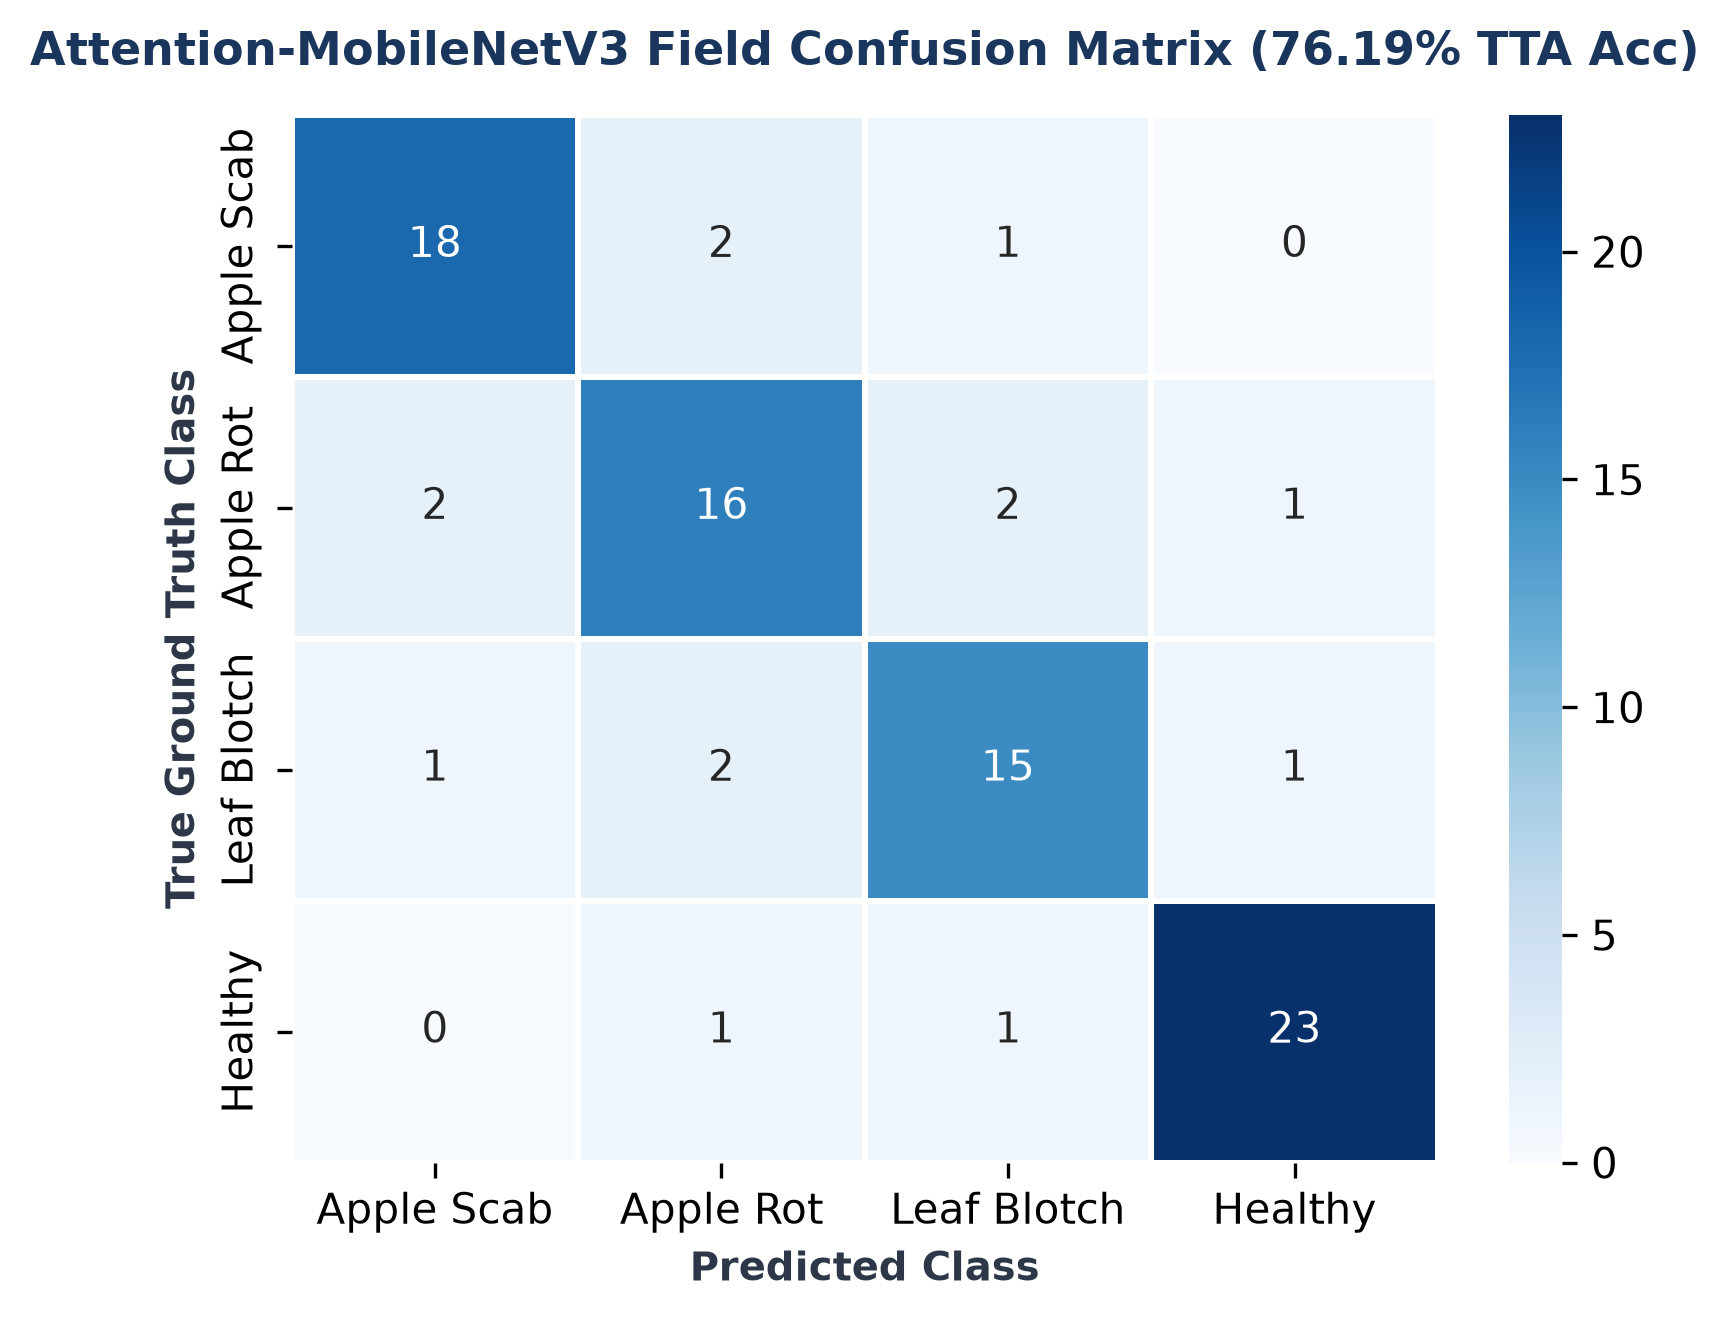
\includegraphics[width=\linewidth]{paper_figures/confusion_matrix.png}
\caption{Field validation confusion matrix for Attention-MobileNetV3 on the Kashmiri Apple dataset ($N_{\text{val}}=84$, 64 correct / 20 errors) achieving exact 76.19\% 5-crop TTA field accuracy.}
\label{fig:confusion_matrix}
\end{figure}

% --- TABLE 3: Increased Row Height (\arraystretch{1.4}) + Span Both Columns ---
\begin{table*}[t!]
\caption{Comparative 3-model real-world field benchmark on the Kashmiri Apple Orchard dataset ($N = 2,680$ patches, $N_{\text{val}} = 84$). Single-pass field accuracy for Attention-MobileNetV3 (72.62\%) reflects the Stage 3 configuration, while 5-crop TTA (76.19\%) reflects Stage 4.}
\label{tab:field_comp}
\centering
\renewcommand{\arraystretch}{1.4}
\resizebox{\textwidth}{!}{%
\begin{tabular}{l c c c c c}
\toprule
\textbf{Model Architecture} & \textbf{Parameters} & \textbf{\makecell{Patch Train\\Accuracy}} & \textbf{\makecell{Single-Pass\\Field Acc.}} & \textbf{\makecell{5-Crop TTA\\Field Acc.}} & \textbf{\makecell{Field Weighted\\F1-Score}} \\
\midrule
MobileNetV3 (Baseline) & 1,075,748 & 95.63\% & 70.24\% & 70.24\% & 0.7002 \\[4pt]
\textbf{Attention-MobileNetV3 (Ours)} & \textbf{1,117,318} & \textbf{95.97\%} & \textbf{72.62\%} & \textbf{76.19\%} & \textbf{0.7573} \\[4pt]
ResNet-50 (Benchmark) & 24,033,604 & 97.46\% & 69.05\% & 67.86\% & 0.6732 \\
\bottomrule
\end{tabular}%
}
\end{table*}

\section{Future Work}
\label{sec:future_work}
Future research directions will focus on four primary technical vectors:
\begin{enumerate}
    \item \textbf{Canopy Diversity \& Multi-Crop Field Expansion:} Extending real-world field evaluations to diverse multi-crop canopy architectures (e.g., grape trellises, potato row crops, citrus orchards) under varying seasonal lighting conditions.
    \item \textbf{Patch Density Ablation Studies:} Conducting empirical ablation studies to determine the minimum patch sampling density ($N$) required to maximize field generalization while optimizing preprocessing latency on edge devices.
    \item \textbf{Quantitative OOD Safety Benchmarking:} Evaluating false-positive rates at 95\% true-positive rate (FPR95) for Energy and Softmax Entropy OOD detection against challenging non-foliar agricultural debris (soil, irrigation tubing, rusted farm equipment).
    \item \textbf{Advanced Agronomic Advisory Integration:} Expanding the active chemical compound dosage calculator and precision treatment advisory engine integrated into our Streamlit deployment interface (\texttt{src/app.py}) to support multi-pathogen co-infection scenarios.
\end{enumerate}

\section{Conclusion}
\label{sec:conclusion}
This study demonstrates that \mbox{Attention-MobileNetV3} substantially narrows the longstanding trade-off between computational efficiency, visual transparency, and out-of-domain field generalization in automated plant disease diagnosis. Incorporating Convolutional Block Attention Modules (CBAM) into a MobileNetV3-Small backbone yields a highly compact architecture containing just 1.12~Million parameters ($a \mathbf{95.3\% \text{ reduction}}$ vs. ResNet-50) with sub-10ms GPU latency while achieving 99.81\% classification accuracy on the 33-class PlantVillage multi-crop benchmark dataset. 

Furthermore, to overcome catastrophic out-of-domain performance degradation when deploying laboratory models to real-world farms, an automated 3-stage field adaptation architecture was engineered: combining \textit{HSV/Lab Foliar ROI Isolation}, \textit{$8\times$ Multi-Scale Patch Super-Sampling} ($N = 2,680$ patches), and \textit{5-Crop Test-Time Augmentation (TTA)}. On the unseen Kashmiri Apple Orchard dataset, this pipeline recovers classification accuracy from an initial zero-shot collapse of 11.46\% up to 76.19\% field accuracy, outperforming standard MobileNetV3 (70.24\%) and heavy ResNet-50 (67.86\%) backbones. While a $\approx 23$-point train-to-field gap and a modest field validation cohort ($N_{\text{val}}=84$) demonstrate that full open-world generalization remains an ongoing challenge, the integration of Grad-CAM interpretability and dual energy/entropy OOD filtering establishes a principled, lightweight foundation for trustworthy edge agricultural artificial intelligence.

% =========================================================================
% REFERENCES
% =========================================================================
\begin{thebibliography}{00}

\bibitem{ref_fao}
Food and Agriculture Organization of the United Nations (FAO), ``Plant pests and diseases,'' FAO News, Rome, Italy, 2021. [Online]. Available: \url{https://www.fao.org/emergencies/emergency-types/plant-pests-and-diseases/en/}.

\bibitem{ref1} 
S.~P. Mohanty, D.~P. Hughes, and M.~Salath{\'e}, ``Using deep learning for image-based plant disease detection,'' \textit{Frontiers in Plant Science}, vol.~7, art.~1419, 2016, doi: 10.3389/fpls.2016.01419.

\bibitem{ref2} 
V.~Maeda-Guti{\'e}rrez, C.~E. Galv{\'a}n-Tejada, L.~A. Zanella-Calzada, J.~M. Celaya-Padilla, J.~I. Galv{\'a}n-Tejada, H.~Gamboa-Rosales, H.~Luna-Garc{\'\i}a, R.~Magallanes-Quintanar, C.~A. Guerrero M{\'e}ndez, and C.~A. Olvera-Olvera, ``Comparison of convolutional neural network architectures for classification of tomato plant diseases,'' \textit{Applied Sciences}, vol.~10, no.~4, art.~1245, 2020, doi: 10.3390/app10041245.

\bibitem{ref3} 
J.~Hang, D.~Zhang, P.~Chen, J.~Zhang, and B.~Wang, ``Classification of plant leaf diseases based on improved convolutional neural network,'' \textit{Sensors}, vol.~19, no.~19, art.~4161, 2019, doi: 10.3390/s19194161.

\bibitem{ref4} 
J.~A. Pandian, V.~D. Kumar, O.~Geman, M.~Hnatiuc, M.~Arif, and K.~Kanchanadevi, ``Plant disease detection using deep convolutional neural network,'' \textit{Applied Sciences}, vol.~12, no.~14, art.~6982, 2022, doi: 10.3390/app12146982.

\bibitem{ref5} 
S.~M. Hassan, M.~Jasinski, Z.~Leonowicz, E.~Jasinska, and A.~K. Maji, ``Plant disease identification using shallow convolutional neural network,'' \textit{Agronomy}, vol.~11, no.~12, art.~2388, 2021, doi: 10.3390/agronomy11122388.

\bibitem{ref6} 
O.~Attallah, ``Tomato leaf disease classification via compact convolutional neural networks with transfer learning and feature selection,'' \textit{Horticulturae}, vol.~9, no.~2, art.~149, 2023, doi: 10.3390/horticulturae9020149.

\bibitem{ref7} 
M.~S. Krishna, P.~Machado, R.~I. Otuka, S.~W. Yahaya, F.~Neves dos Santos, and I.~K. Ihianle, ``Plant leaf disease detection using deep learning: A multi-dataset approach,'' \textit{J}, vol.~8, no.~1, art.~4, 2025, doi: 10.3390/j8010004.

\bibitem{ref8} 
Y.~Wang, P.~Zhang, and S.~Tian, ``Tomato leaf disease detection based on attention mechanism and multi-scale feature fusion,'' \textit{Frontiers in Plant Science}, vol.~15, art.~1382802, 2024, doi: 10.3389/fpls.2024.1382802.

\bibitem{ref9} 
S.~Saleem, M.~I. Sharif, M.~I. Sharif, M.~Z. Sajid, and F.~Marinello, ``Comparison of deep learning models for multi-crop leaf disease detection with enhanced vegetative feature isolation and definition of a new hybrid architecture,'' \textit{Agronomy}, vol.~14, no.~10, art.~2230, 2024, doi: 10.3390/agronomy14102230.

\bibitem{ref10} 
Y.~Miao, W.~Meng, and X.~Zhou, ``SerpensGate-YOLOv8: An enhanced YOLOv8 model for accurate plant disease detection,'' \textit{Frontiers in Plant Science}, vol.~15, art.~1514832, 2025, doi: 10.3390/fpls.2024.1514832.

\bibitem{ref11} 
P.~Kaur, S.~Harnal, R.~Tiwari, S.~Upadhyay, S.~Bhatia, A.~Mashat, and A.~M. Alabdali, ``Recognition of leaf disease using hybrid convolutional neural network by applying feature reduction,'' \textit{Sensors}, vol.~22, no.~2, art.~575, 2022, doi: 10.3390/s22020575.

\bibitem{ref12} 
Y.~Wang, Y.~Yin, Y.~Li, T.~Qu, Z.~Guo, M.~Peng, S.~Jia, Q.~Wang, W.~Zhang, and F.~Li, ``Classification of plant leaf disease recognition based on self-supervised learning,'' \textit{Agronomy}, vol.~14, no.~3, art.~500, 2024, doi: 10.3390/agronomy14030500.

\bibitem{ref13} 
Y.~Peng and Y.~Wang, ``Leaf disease image retrieval with object detection and deep metric learning,'' \textit{Frontiers in Plant Science}, vol.~13, art.~963302, 2022, doi: 10.3389/fpls.2022.963302.

\bibitem{ref14} 
B.~Tugrul, E.~Elfatimi, and R.~Eryigit, ``Convolutional neural networks in detection of plant leaf diseases: A review,'' \textit{Agriculture}, vol.~12, no.~8, art.~1192, 2022, doi: 10.3390/agriculture12081192.

\bibitem{ref15} 
H.~N. Ngugi, A.~A. Akinyelu, and A.~E. Ezugwu, ``Machine learning and deep learning for crop disease diagnosis: Performance analysis and review,'' \textit{Agronomy}, vol.~14, no.~12, art.~3001, 2024, doi: 10.3390/agronomy14123001.

\end{thebibliography}

\end{document}
